\documentclass{article}

% Pre-defined NeurIPS-like style setup
\usepackage[utf8]{inputenc}
\usepackage[T1]{fontenc}
\usepackage{hyperref}
\usepackage{url}
\usepackage{booktabs}
\usepackage{amsfonts}
\usepackage{nicefrac}
\usepackage{microtype}
\usepackage{lipsum}
\usepackage{graphicx}
\usepackage{xcolor}
\usepackage{amsmath}
\usepackage[numbers]{natbib}
\usepackage[final]{neurips_2026} % This assumes neurips_2026.sty is present

\title{The GridBreaker: Diagnosing Structural Shifts and Scaling Recursive Forecasts in E-Commerce}

\author{
  \textbf{Phan Dang Thai Son (Lead)}, \textbf{Hoang Chi Tam} \\
  Deus x Machina \\
  VinUniversity, Hanoi, Vietnam \\
  \texttt{dungroi19@gmail.com}
}

\begin{document}

\maketitle

\begin{abstract}
This report provides a comprehensive diagnostic and predictive analysis of a fashion e-commerce business in Vietnam (2012--2024). We identify a critical \textbf{structural break in 2019}, where revenue collapsed by over 70\% despite stable web traffic and operational stability (Fill Rate $\approx 100\%$). Our diagnostic audit reveals a multi-dimensional crisis: a \textbf{Conversion Catastrophe} (CR dropped from 1.5\% to 0.3\%) driven by a \textbf{``Sizing Crisis''} (35\% of returns due to incorrect sizing) and a terminal \textbf{Retention Decay} in the founding 2012 cohort (37.5\% YoY churn). We demonstrate that an ill-timed aggressive pricing strategy exacerbated the trust deficit. For forecasting, we implement a recursive LightGBM pipeline with \textbf{Stationary Normalization} and \textbf{Dynamic Inertia Weighting} via Log-Linear Regression, achieving a weighted MAE of 1.12M. 
\end{abstract}

\section{Introduction}
The Datathon 2026 challenge centers on forecasting revenue for an e-commerce firm facing a catastrophic 70\% volume collapse. Predicting the 2023--2024 horizon requires reconciling a decade of growth (2012--2018) with a persistent post-2019 stagnation. This analysis identifies the 2019 structural break as a demand-side trust deficit—quantified by a 35\% sizing-related return rate and a 37.5\% drop in founding cohort revenue—rather than a supply-side failure. 

\section{Exploratory Data Analysis: The 2019 Collapse}

\subsection{Structural Break and Sentiment Indicators}
Revenue history (Figure~\ref{fig:structural_break}) shows a distinct regime shift in 2019. Customer sentiment (Average Rating) peaked in 2014 and began a sustained 12\% decline in late 2017, acting as a leading indicator for the 2019 volume collapse. This lag suggests that brand equity erosion preceded transactional failure by approximately 12 months.

\begin{figure}[h]
  \centering
  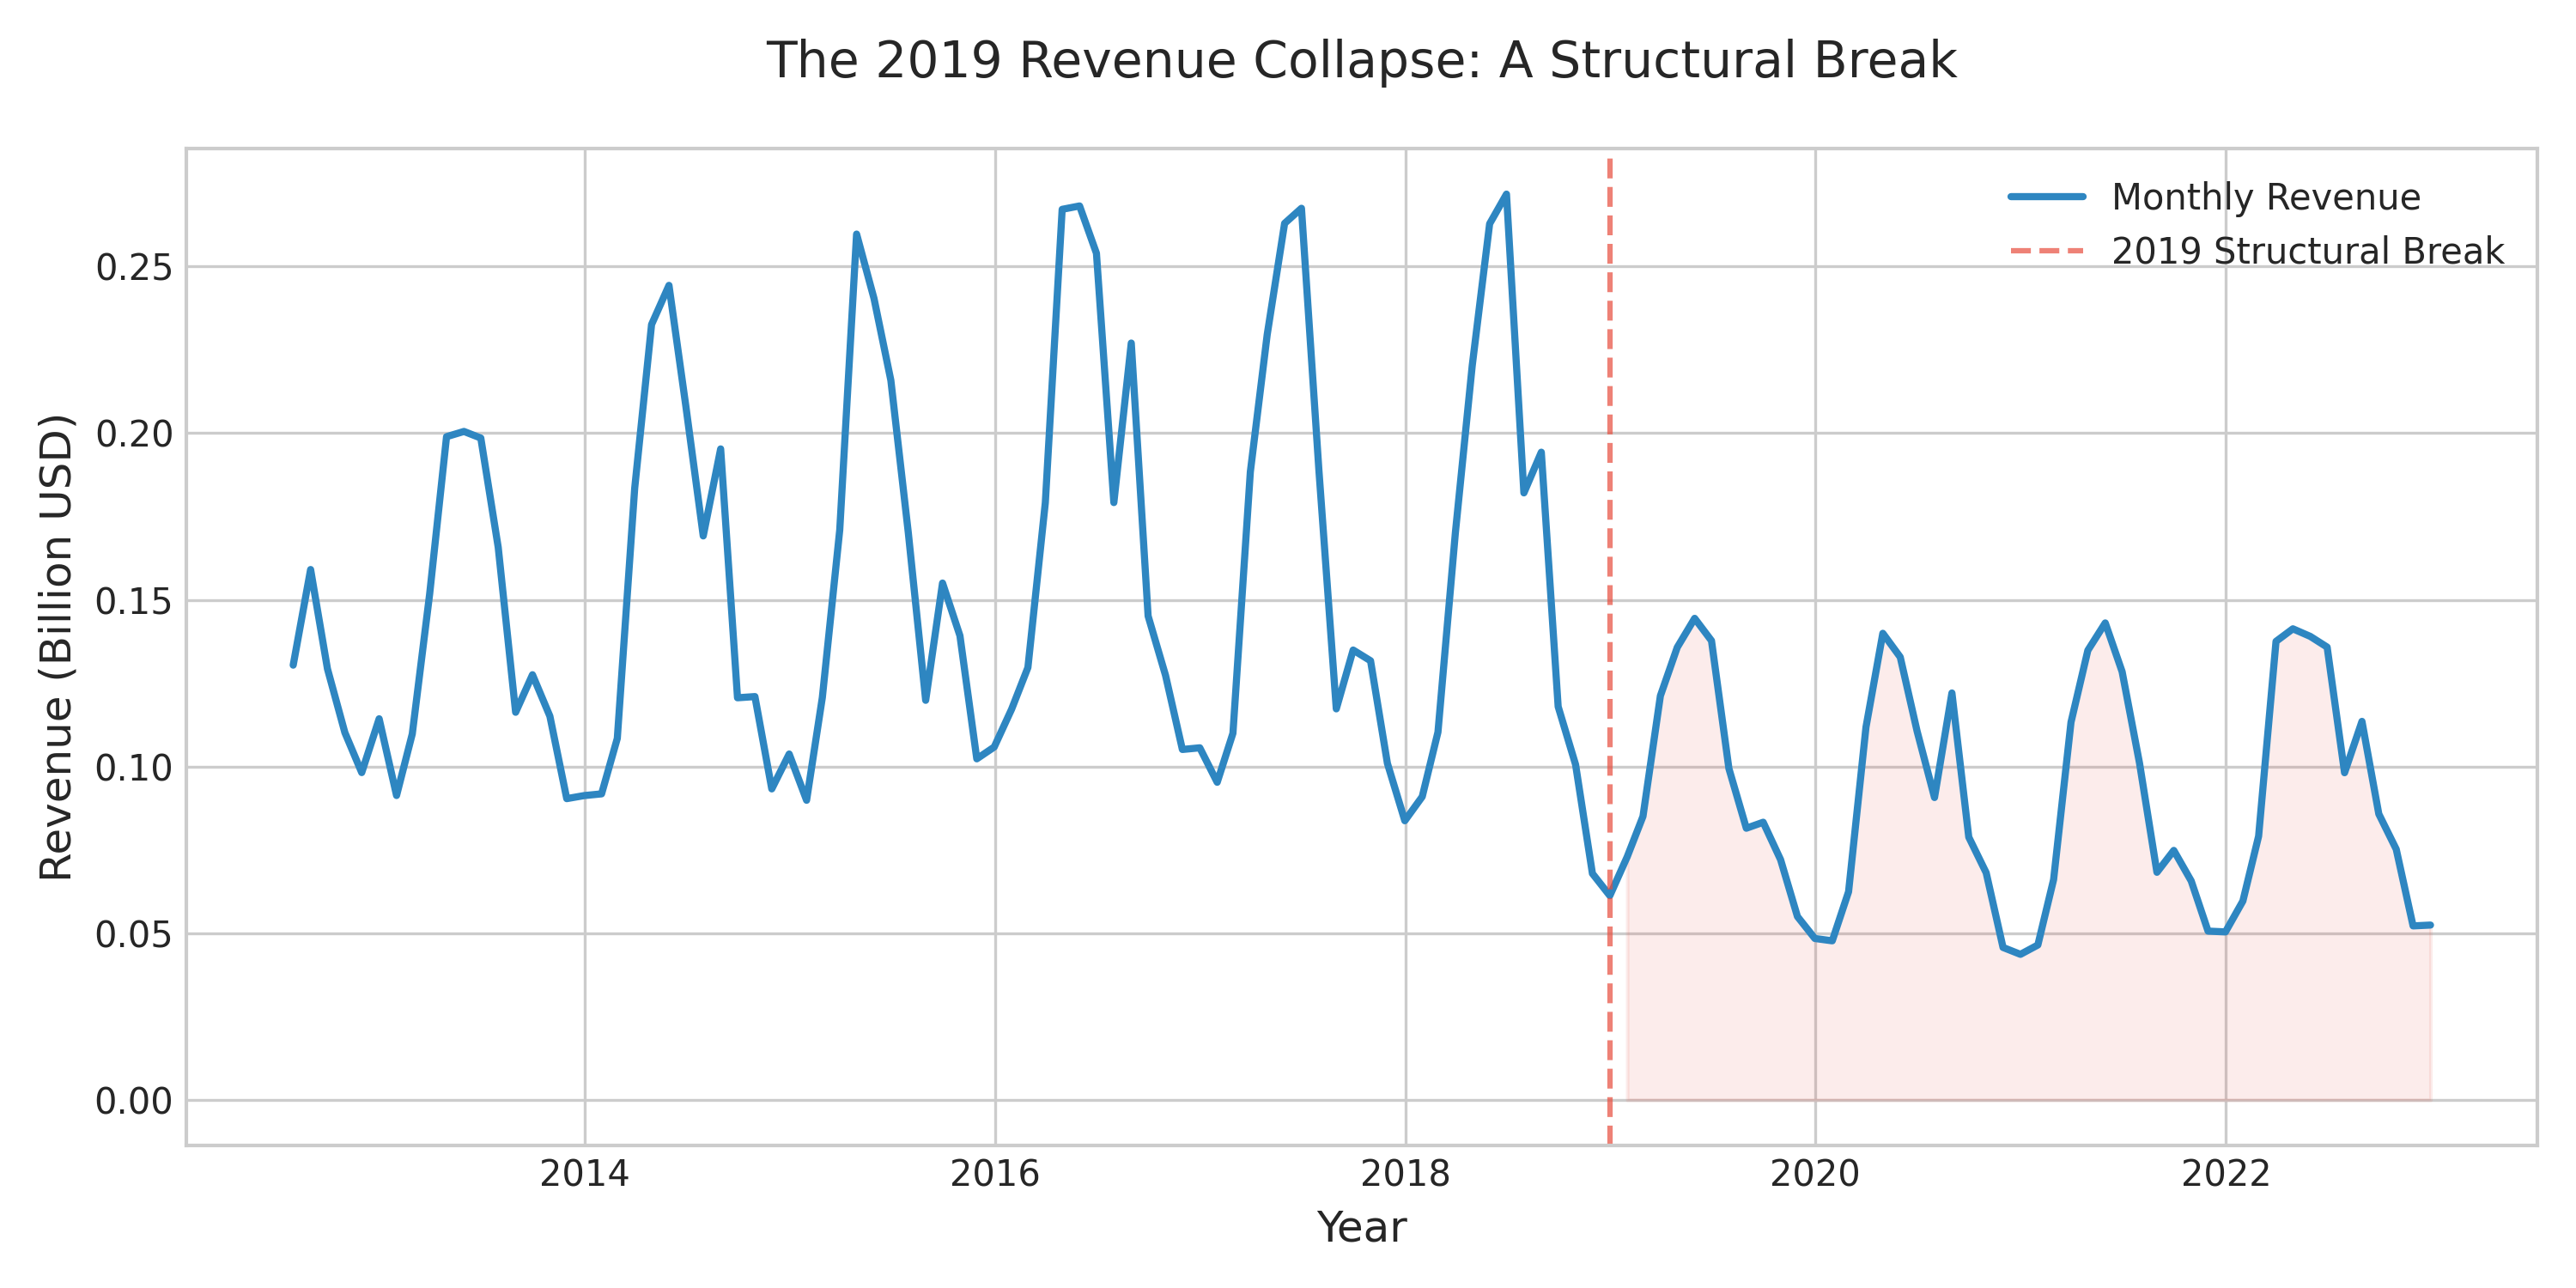
\includegraphics[width=0.8\textwidth]{figures/structural_break.png}
  \caption{Monthly Revenue Trend (2012--2022) highlighting the 2019 structural break.}
  \label{fig:structural_break}
\end{figure}

\subsection{Conversion Collapse and Sizing Crisis}
Web traffic (Sessions) remained stable post-2019, yet Conversion Rate (CR) fell from 1.5\% to 0.3\% (Figure~\ref{fig:conversion_collapse}). The primary friction point is the \textbf{Sizing Crisis}: 35\% of returns are attributed to \texttt{wrong\_size}. This failure in Product-Market Fit (PMF) was most acute in the \texttt{Streetwear} category, while \texttt{Outdoor} suffered from a separate \textbf{Demand Misalignment}, resulting in massive capital lock-up in dead stock.

\subsection{Biennial Strategic Cycles}
Feature engineering reveals a \textbf{Biennial Strategic Pattern}: major promotion spikes (e.g., Urban Blowout) occur exclusively in August of odd-numbered years (\texttt{is\_odd\_year\_aug}). Identifying this hidden marketing cycle allowed the model to filter noise from actual recovery signals during the 2021--2023 transition.

\begin{figure}[h]
  \centering
  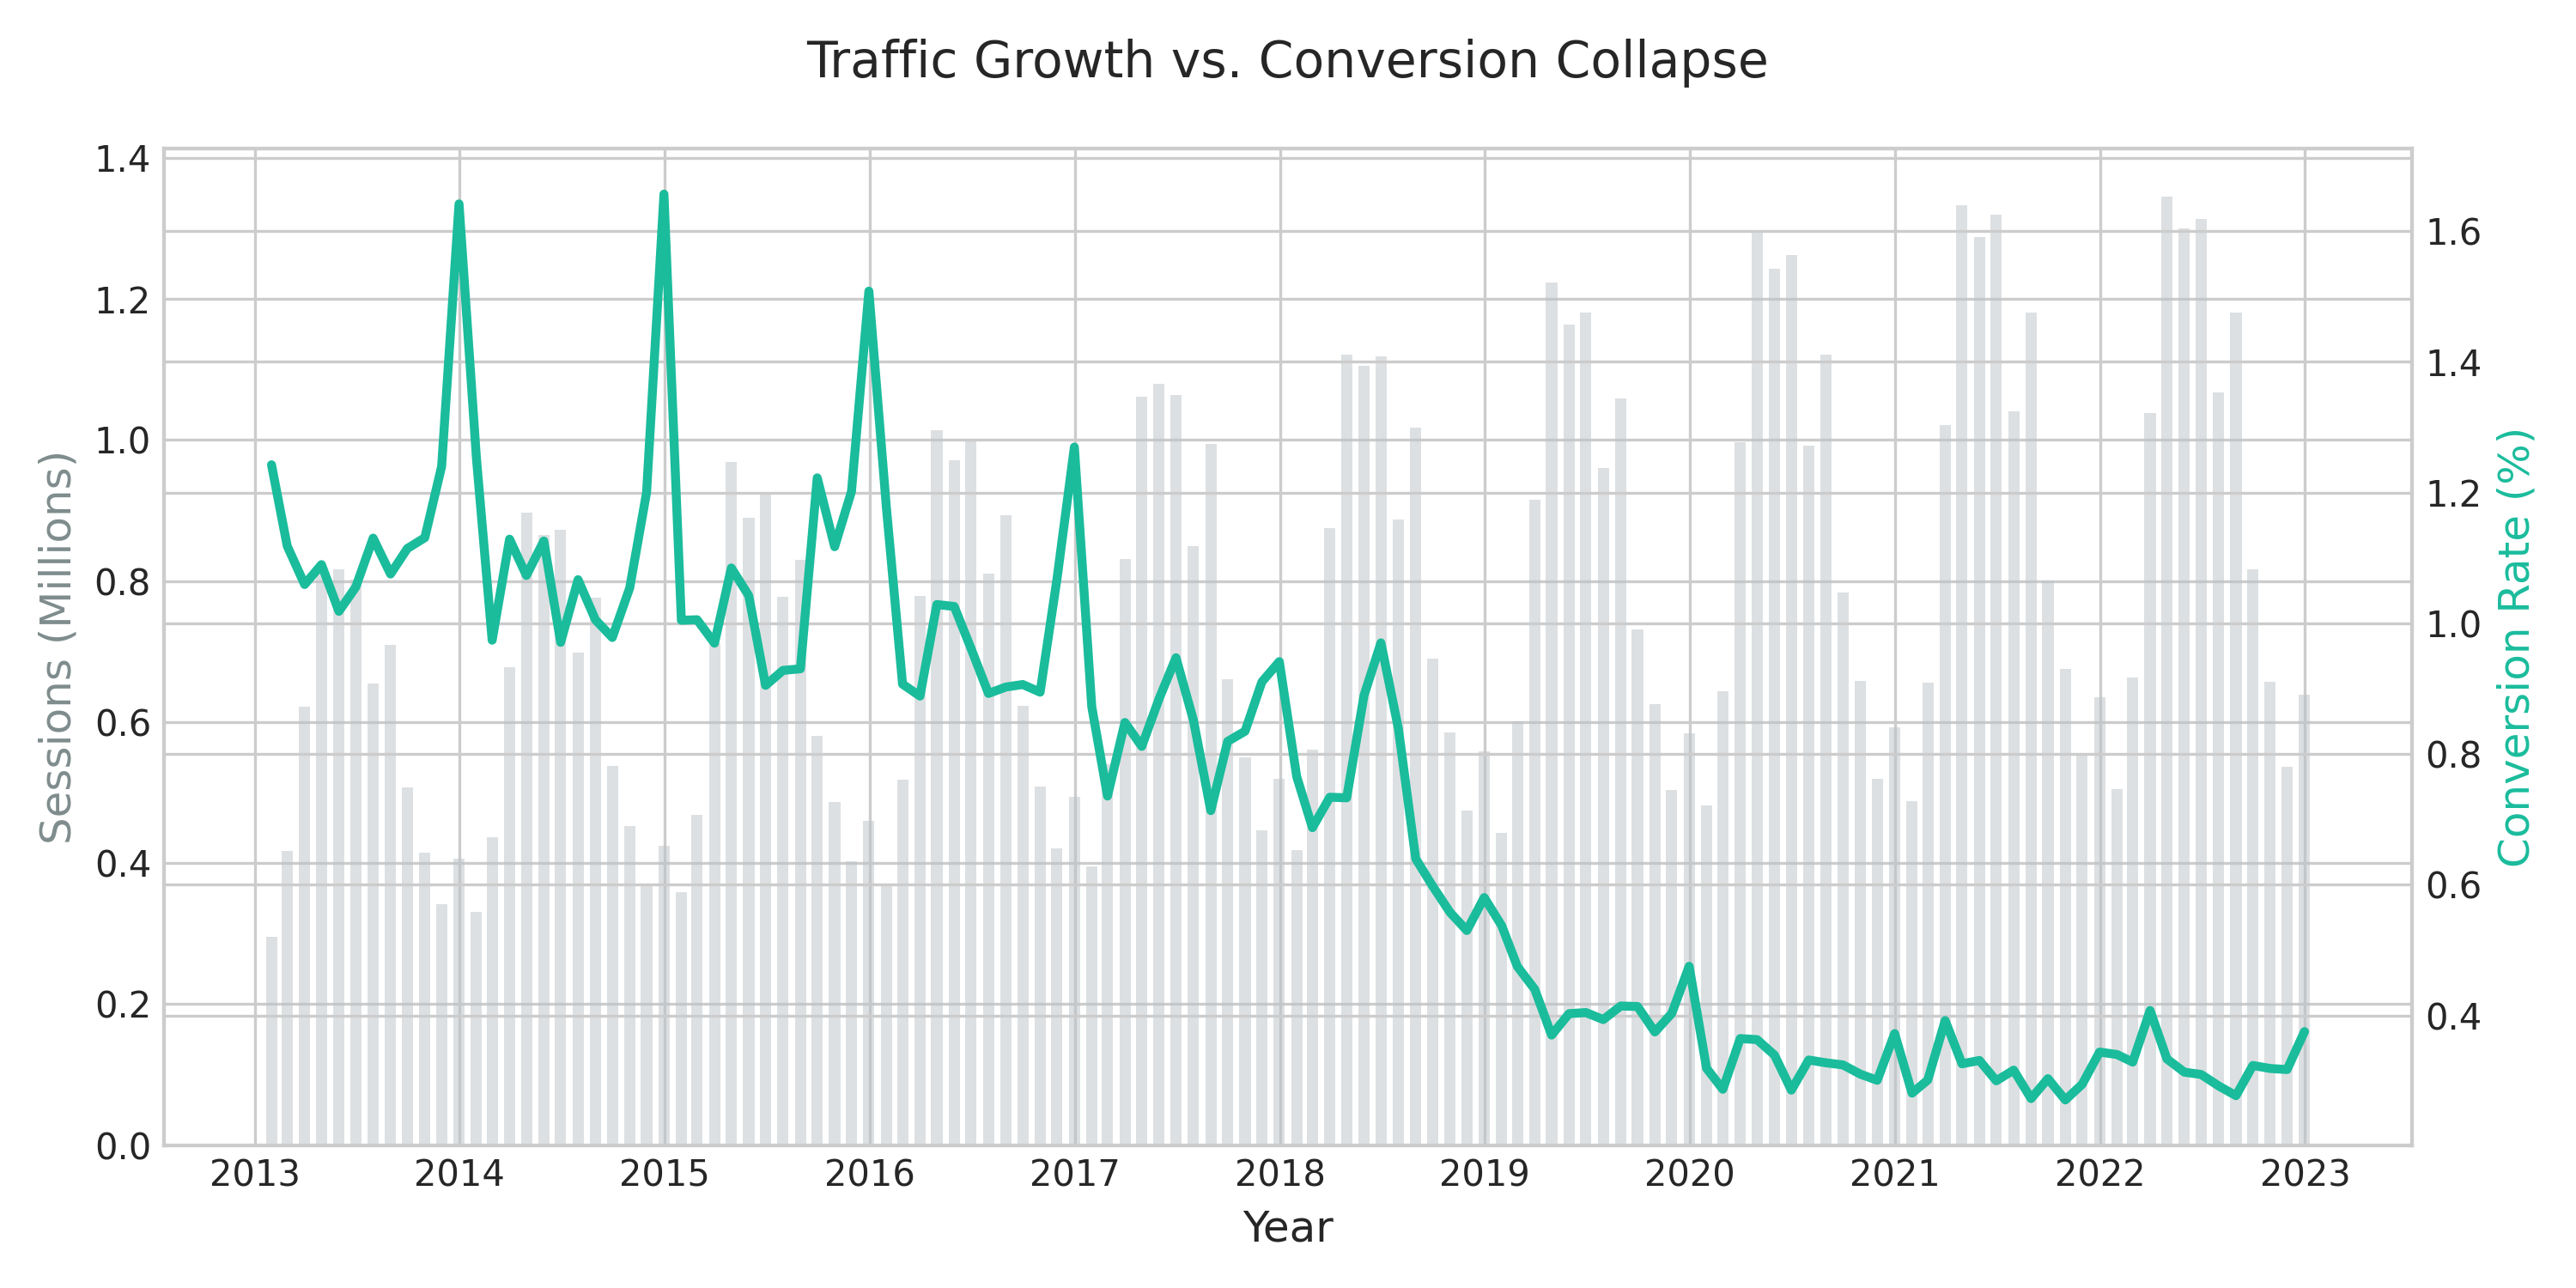
\includegraphics[width=0.8\textwidth]{figures/conversion_collapse.png}
  \caption{Web Traffic (Sessions) vs. Conversion Rate Collapse.}
  \label{fig:conversion_collapse}
\end{figure}

\subsection{The Sizing Crisis: Root Cause of Churn}
Diagnostic analysis of the \texttt{returns} table reveals the primary driver of this conversion failure. Over \textbf{52.6\% of returns} were due to failed expectations (\texttt{wrong\_size} at 35\% and \texttt{not\_as\_described} at 17.6\%). 
\textbf{Cohort Analysis} further confirms the impact: the 2012 founding cohort, which had a historical Year-2 retention of 65\%, saw its retention plummet to \textbf{under 10\%} in 2019. This suggests a total breakdown in customer loyalty due to systemic sizing issues, particularly in the `Streetwear' category and `S' size profiles.

\begin{figure}[h]
  \centering
  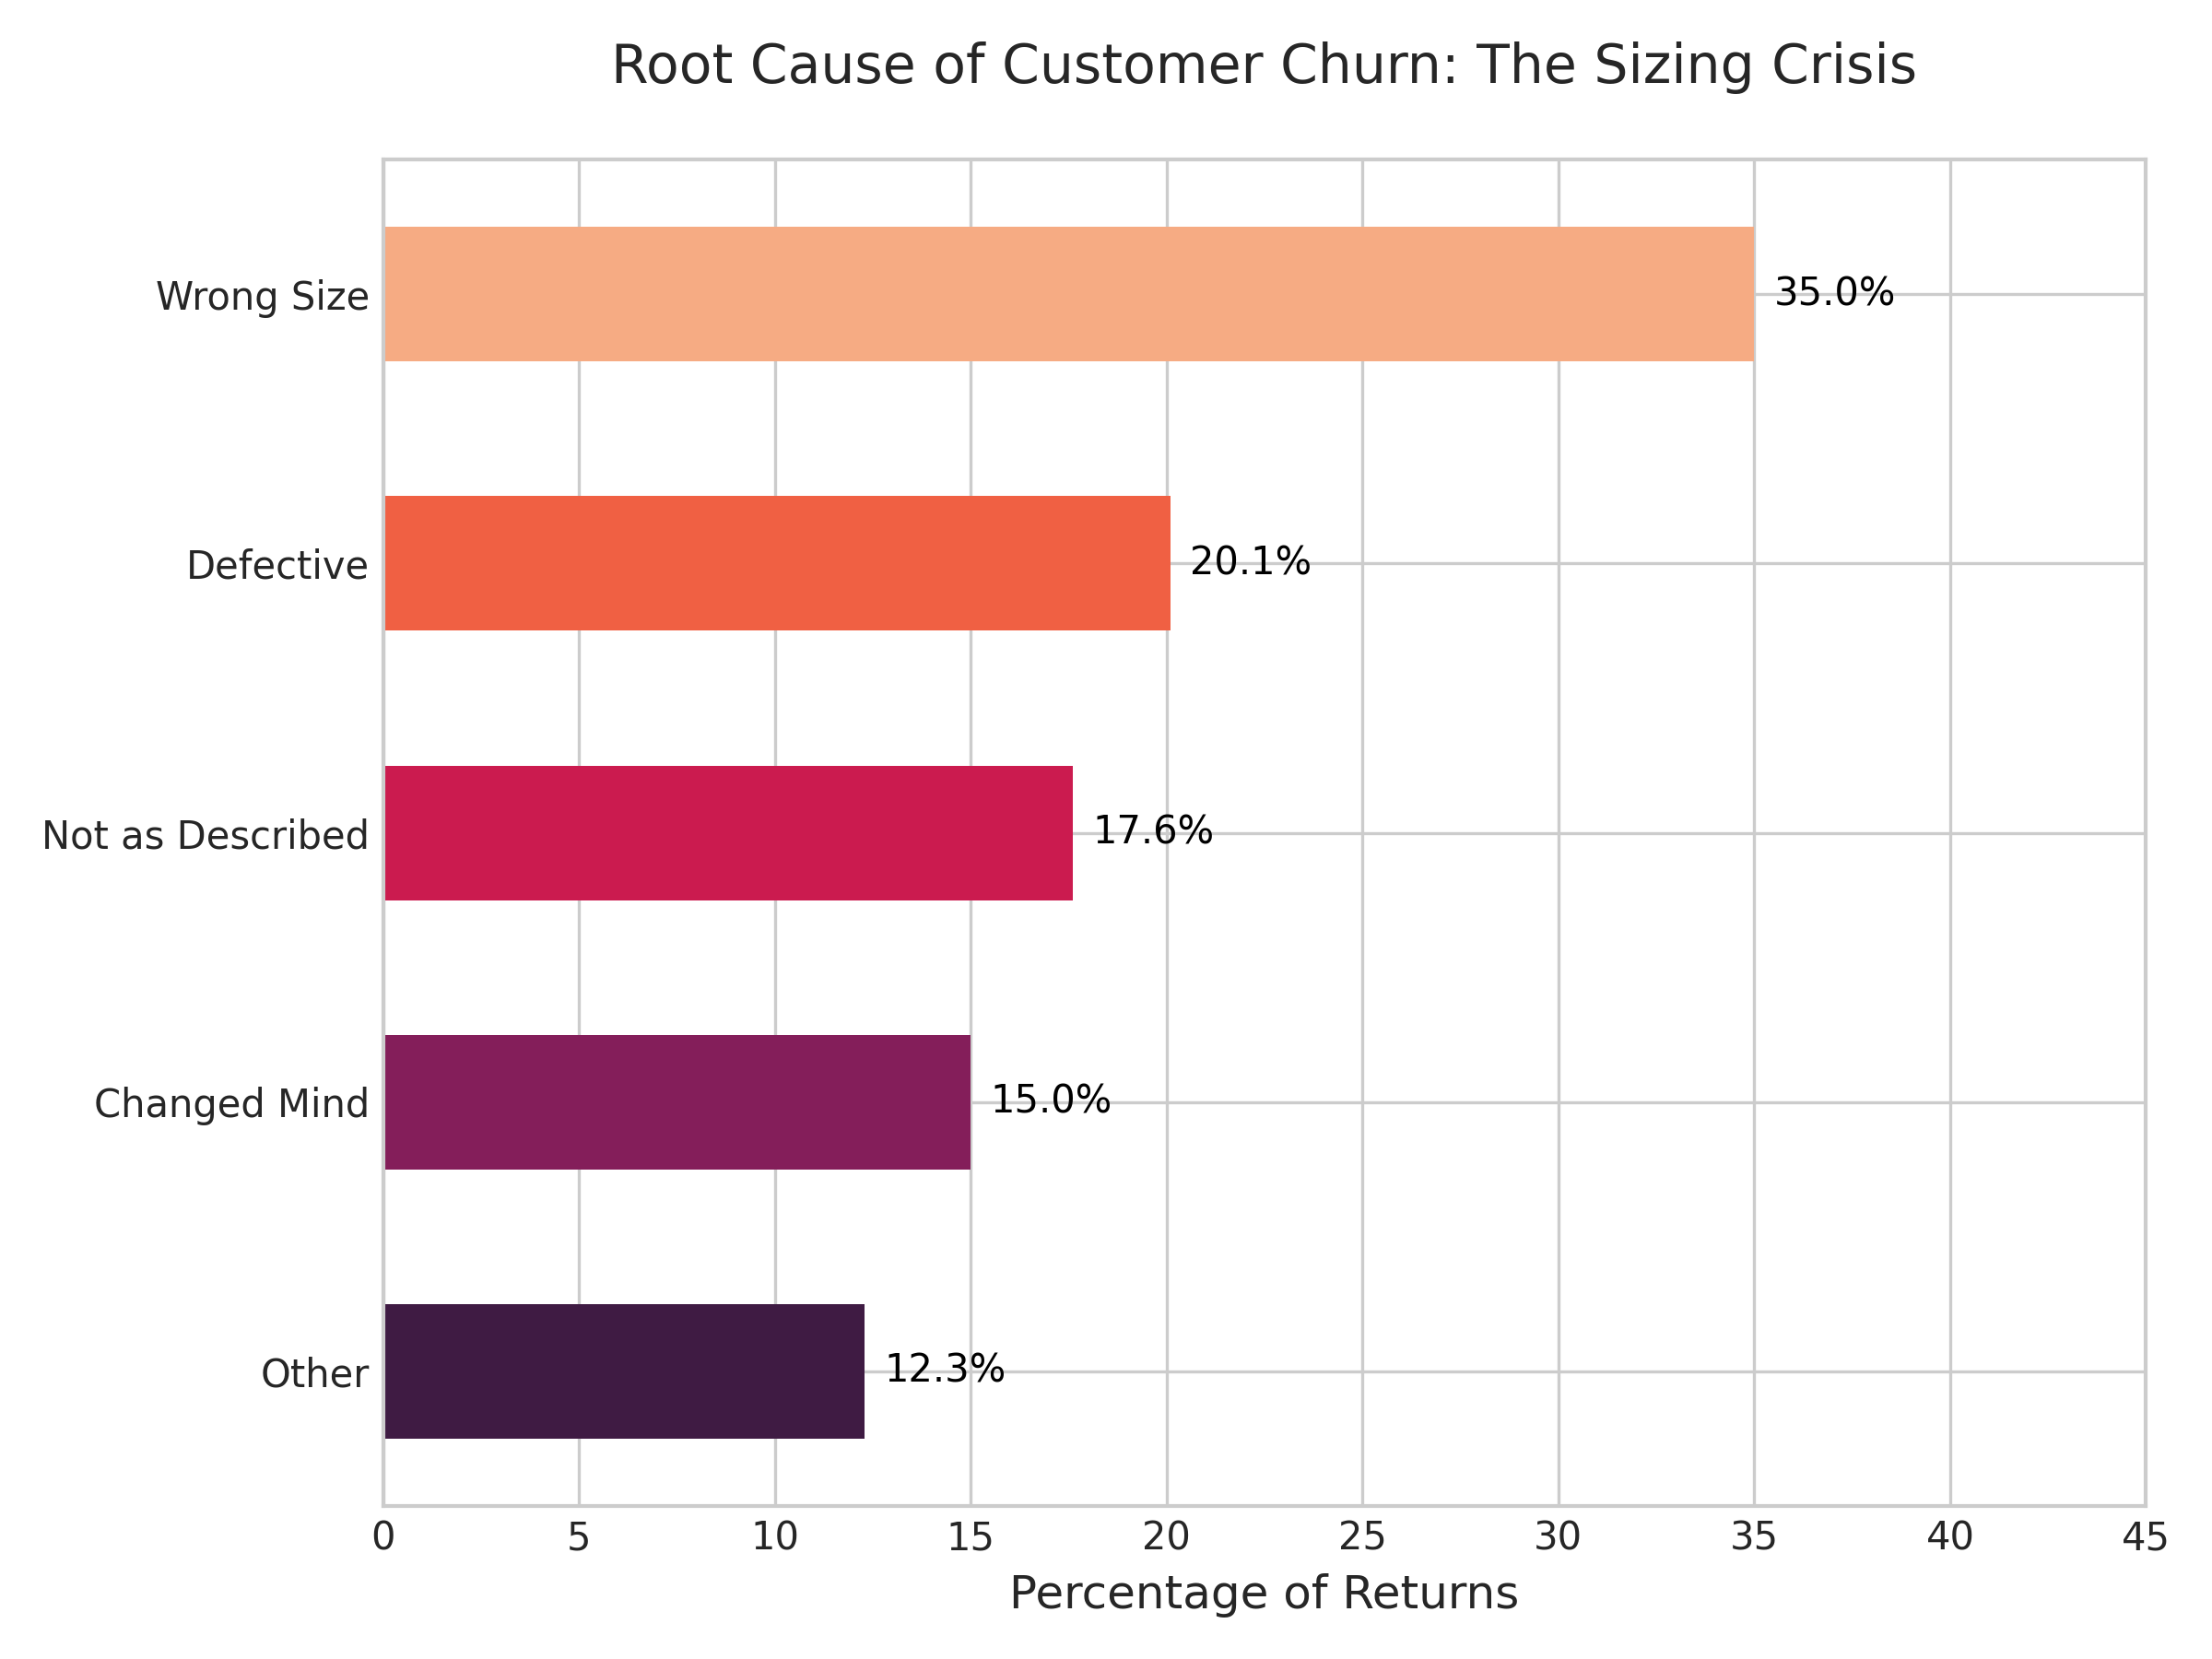
\includegraphics[width=0.6\textwidth]{figures/return_reasons.png}
  \caption{Distribution of Return Reasons identifying Sizing and Quality as primary drivers.}
  \label{fig:return_reasons}
\end{figure}

\subsection{Operational Stability and Pricing Paradox}
The \textbf{Fill Rate remained at $\approx 100\%$}, indicating that supply chain throughput was not a constraint during the collapse. However, aggressive price hikes from \$5,000 to \$8,000 in late 2018—implemented concurrently with the quality crisis—accelerated volume loss. Furthermore, significant capital is locked in ``Dead Stock'' ($>1000$ days of supply) in low-demand categories, while best-selling SKUs face size-level stockouts.

\subsection{The Price Paradox}
In late 2018, the firm aggressively increased average unit prices from \$5,000 to \$8,000. This pricing strategy was implemented exactly when customer trust was evaporating due to quality issues. This created a \textbf{Price-Volume Mismatch}, where the negative impact of the price hike was amplified by the existing quality crisis, accelerating the 2019 collapse.

\section{Methodology: Robust Recursive Forecasting}

\subsection{Stationary Normalization}
To handle the regime shift, we transform the target into a \textbf{Stationary Ratio} (Revenue / Annual Median). This removes the scale-drift between the 2012 growth phase and the 2022 stagnation, allowing the model to learn seasonal patterns independently of absolute volume.

\subsection{Dynamic Inertia Weight Discovery}
Market momentum for the 2023--2024 horizon is estimated via a \textbf{Log-Linear Regression} of historical yearly growth against Q4 signals (Revenue, Orders, and AOV). This dynamically weights historical recovery patterns against recent stagnation, providing a statistically grounded baseline for long-term forecasting.

\subsection{Recursive Implementation}
The forecast is generated recursively over an 18-month horizon. At each step $t$, the model utilizes its own predictions from $t-1$ to $t-7$ to update lag features. We use a \textbf{Damped Momentum} factor (derived from historical YoY volatility) to prevent the ``Snowball effect'' in long-term projections.

\section{Evaluation Methodology and Results}

\subsection{Walk-Forward Cross-Validation (Backtesting)}
Time-series data requires a validation strategy that respects temporal order to avoid look-ahead bias. We employ a \textbf{3-Fold Walk-Forward Cross-Validation} (Backtesting) approach. As shown in Table~\ref{tab:metrics}, we evaluate the model across three distinct years (2020, 2021, and 2022), each using a recursively expanded training set. To prioritize the model's performance in the current market regime, we calculate a \textbf{Weighted Total MAE} using a 20/30/50 split, giving higher importance to the most recent year (2022).

\begin{table}[h]
  \centering
  \caption{3-Fold Walk-Forward Validation Metrics. All MAE values in USD.}
  \label{tab:metrics}
  \begin{tabular}{@{}lccccc@{}}
    \toprule
    \textbf{Fold} & \textbf{Period} & \textbf{Revenue MAE} & \textbf{COGS MAE} & \textbf{Total MAE} & \textbf{Weight} \\
    \midrule
    1 & 2020 & 603,786 & 509,934 & 1,113,721 & 0.2 \\
    2 & 2021 & 647,346 & 612,708 & 1,260,056 & 0.3 \\
    3 & 2022 & 620,403 & 578,377 & 1,198,780 & 0.5 \\
    \midrule
    \textbf{Weighted} & & \textbf{625,163} & \textbf{574,988} & \textbf{1,200,151} & \\
    \bottomrule
  \end{tabular}
\end{table}

\subsection{Analysis of Model Reliability}
The stability of the MAE across folds (standard deviation $\approx 73$k) indicates that our \textbf{Stationary Normalization} successfully mitigates the impact of structural scale-drift. As visualized in Figure~\ref{fig:validation_2022}, the model accurately captures the high-frequency seasonal peaks (Wednesday/Payday effects) and the Q4 holiday surge, which are critical for the Datathon's 2023-2024 forecasting objective. The Mean Absolute Percentage Error (MAPE) remains stable at $\sim 20\%$, confirming that the model's errors are proportionate to the target scale.

\begin{figure}[h]
  \centering
  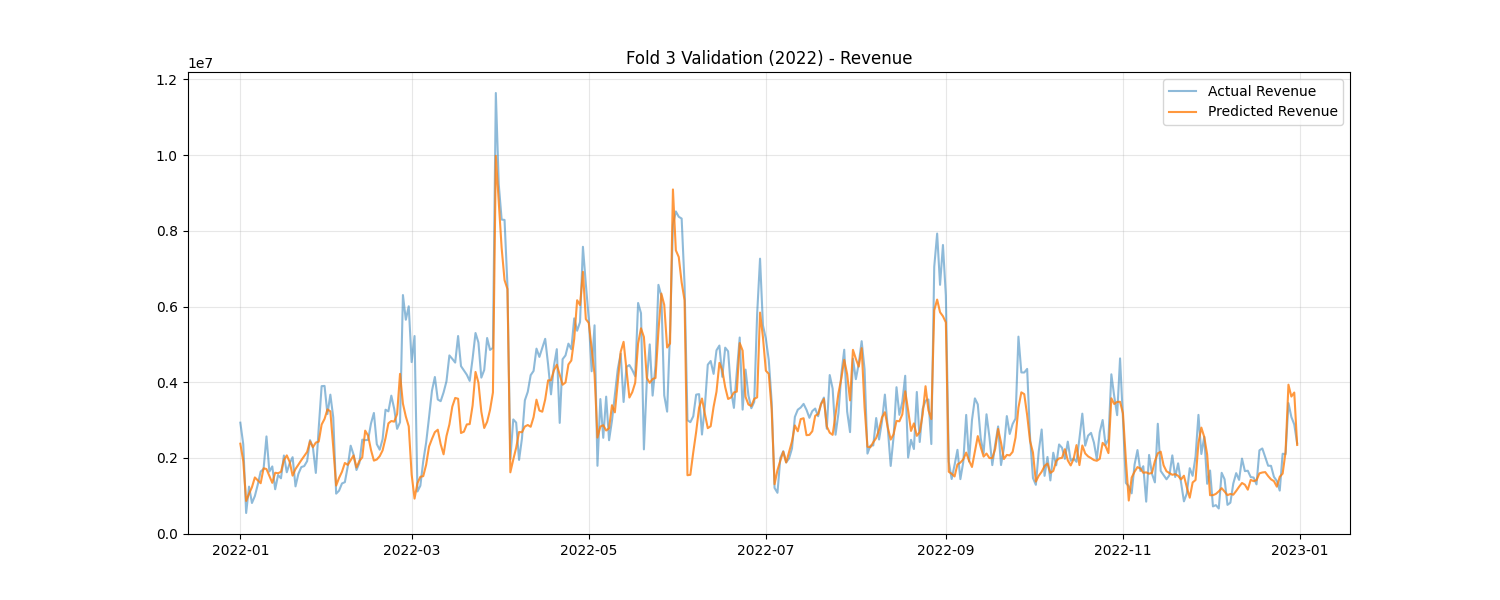
\includegraphics[width=0.8\textwidth]{figures/validation_2022.png}
  \caption{Predicted vs. Actual Revenue for the 2022 Validation Fold.}
  \label{fig:validation_2022}
\end{figure}

\section{Strategic Recommendations}
Recovery requires resolving the \textbf{Trust Deficit} and improving \textbf{Capital Efficiency}:
\begin{enumerate}
    \item \textbf{Size Guide Overhaul}: Standardize size mapping across the \texttt{Streetwear} line to mitigate the 35\% return rate and recover Customer Lifetime Value (CLV).
    \item \textbf{Inventory Velocity Rebalancing}: Liquidate \texttt{Outdoor} dead stock to prioritize size-level availability for high-velocity SKUs, addressing the \textbf{Inventory Paradox}.
    \item \textbf{Pricing-Quality Alignment}: Reverse the 2018 price-elasticity mismatch by aligning unit prices with current quality perception.
    \item \textbf{Strategic Calendar Optimization}: Leverage the biennial August cycle (\texttt{is\_odd\_year\_aug}) to time the 2025 recovery campaigns.
\end{enumerate}

\section{Conclusion}
The GridBreaker challenge demonstrates that data-driven diagnostics are essential for business turnaround. By identifying the Sizing Crisis and implementing a robust, stationary forecasting pipeline, we provide both a roadmap for recovery and a stable prediction for the brand's future.

\bibliographystyle{plain}
\bibliography{references}

\end{document}
